% !TeX spellcheck = en_US
%% 字体:方正静蕾简体
%%		 方正粗宋
\documentclass[a4paper,left=2.5cm,right=2.5cm,11pt]{article}
\usepackage[utf8]{inputenc}
\usepackage{fontspec}
\usepackage{cite}
\usepackage{xeCJK}
\usepackage{indentfirst}
\usepackage{titlesec}
\usepackage{longtable}
\usepackage{graphicx}
\usepackage{float}
\usepackage{rotating}
\usepackage{subfigure}
\usepackage{tabu}
\usepackage{amsmath}
\usepackage{setspace}
\usepackage{amsfonts}
\usepackage{appendix}
\usepackage{listings}
\usepackage{xcolor}
\usepackage{geometry}
\setcounter{secnumdepth}{4}
\usepackage{mhchem}
\usepackage{multirow}
\usepackage{extarrows}
\usepackage{hyperref}
\usepackage{caption}
\usepackage{color}

\titleformat*{\section}{\LARGE}
\renewcommand\refname{参考文献} %设置参考文献的形状
\renewcommand{\abstractname}{\sihao \cjkfzcs 摘{  }要}
%\titleformat{\chapter}{\centering\bfseries\huge\wryh}{}{0.7em}{}{}
%\titleformat{\section}{\LARGE\bf}{\thesection}{1em}{}{}
\titleformat{\subsection}{\Large\bfseries}{\thesubsection}{1em}{}{}
\titleformat{\subsubsection}{\large\bfseries}{\thesubsubsection}{1em}{}{}
\renewcommand{\contentsname}{{\cjkfzcs \centerline{目{  } 录}}}

\setCJKfamilyfont{cjkfzcs}{STSongti-SC-Regular}
% \setCJKfamilyfont{cjkhwxk}{STXingkai}
% \setCJKfamilyfont{cjkhwxk}{华文行楷}
% \setCJKfamilyfont{cjkfzcs}{方正粗宋简体}
\newcommand*{\cjkfzcs}{\CJKfamily{cjkfzcs}}
\newcommand*{\cjkhwxk}{\CJKfamily{cjkhwxk}}
% \newfontfamily\wryh{Microsoft YaHei}
% \newfontfamily\hwzs{STZhongsong}
\newfontfamily\hwst{STSong}
\newfontfamily\hwfs{STFangsong}
% \newfontfamily\jljt{MicrosoftYaHei}
% \newfontfamily\hwxk{STXingkai}
% \newfontfamily\hwzs{华文中宋}
% \newfontfamily\hwst{华文宋体}
% \newfontfamily\hwfs{华文仿宋}
% \newfontfamily\jljt{方正静蕾简体}
% \newfontfamily\hwxk{华文行楷}
\newcommand{\verylarge}{\fontsize{60pt}{\baselineskip}\selectfont}  
\newcommand{\chuhao}{\fontsize{44.9pt}{\baselineskip}\selectfont}  
\newcommand{\xiaochu}{\fontsize{38.5pt}{\baselineskip}\selectfont}  
\newcommand{\yihao}{\fontsize{27.8pt}{\baselineskip}\selectfont}  
\newcommand{\xiaoyi}{\fontsize{25.7pt}{\baselineskip}\selectfont}  
\newcommand{\erhao}{\fontsize{23.5pt}{\baselineskip}\selectfont}  
\newcommand{\xiaoerhao}{\fontsize{19.3pt}{\baselineskip}\selectfont} 
\newcommand{\sihao}{\fontsize{14pt}{\baselineskip}\selectfont}      % 字号设置  
\newcommand{\xiaosihao}{\fontsize{12pt}{\baselineskip}\selectfont}  % 字号设置  
\newcommand{\wuhao}{\fontsize{10.5pt}{\baselineskip}\selectfont}    % 字号设置  
\newcommand{\xiaowuhao}{\fontsize{9pt}{\baselineskip}\selectfont}   % 字号设置  
\newcommand{\liuhao}{\fontsize{7.875pt}{\baselineskip}\selectfont}  % 字号设置  
\newcommand{\qihao}{\fontsize{5.25pt}{\baselineskip}\selectfont}    % 字号设置 

\usepackage{diagbox}
\usepackage{multirow}
\boldmath
\XeTeXlinebreaklocale "zh"
\XeTeXlinebreakskip = 0pt plus 1pt minus 0.1pt
\definecolor{cred}{rgb}{0.8,0.8,0.8}
\definecolor{cgreen}{rgb}{0,0.3,0}
\definecolor{cpurple}{rgb}{0.5,0,0.35}
\definecolor{cdocblue}{rgb}{0,0,0.3}
\definecolor{cdark}{rgb}{0.95,1.0,1.0}
\lstset{   %设置代码的格式
	language=[x86masm]Assembler,
	numbers=left,
	numberstyle=\tiny\color{black},
	showspaces=false,
	showstringspaces=false,
	basicstyle=\scriptsize,
	keywordstyle=\color{purple},
	commentstyle=\itshape\color{cgreen},
	stringstyle=\color{blue},
	frame=lines,
	extendedchars=true, 
	xleftmargin=1em,
	xrightmargin=1em, 
	backgroundcolor=\color{cred},
	aboveskip=1em,
	breaklines=true,
	tabsize=4
} 

\newfontfamily{\monaco}{Monaco}
%\newfontfamily{\consolas}{Consolas}
%\setmonofont[Mapping={}]{Consolas}	%英文引号之类的正常显示,相当于设置英文字体
%\setsansfont{Consolas} %设置英文字体 Monaco, Consolas,  Fantasque Sans Mono
% \setCJKmainfont{华文中宋}
\setmainfont{Times New Roman}

\newcommand{\fic}[1]{\begin{figure}[H]
		\center
		\includegraphics[width=0.8\textwidth]{#1}
	\end{figure}}
	
\newcommand{\sizedfic}[2]{\begin{figure}[H]
		\center
		\includegraphics[width=#1\textwidth]{#2}
	\end{figure}}

\newcommand{\codefile}[1]{\lstinputlisting{#1}}


% 改变段间隔
\setlength{\parskip}{0.6em}
\linespread{1.1}
\usepackage{lastpage}
\usepackage{fancyhdr}
\pagestyle{fancy}

\lhead{\space \qquad \space}
\chead{homework2  \qquad Name:徐晓刚  \qquad Student ID:3140102480 \qquad}
\rhead{\qquad\thepage/\pageref{LastPage}}

\DeclareMathOperator\dif{d\!}


%设置双线页眉
\makeatletter                                         
\def\headrule{{\if@fancyplain\let\headrulewidth\plainheadrulewidth\fi%
		\hrule\@height 1.5pt \@width\headwidth\vskip1pt%上面线为1pt粗  
		\hrule\@height 0.5pt\@width\headwidth  %下面0.5pt粗            
		\vskip-2\headrulewidth\vskip-1.5pt}      %两条线的距离1pt      
	\renewcommand{\headrule}{\hrule depth0pt height0.15truemm width\textwidth}  
	\vspace{6mm}}     %双线与下面正文之间的垂直间距              
\makeatother  

\begin{document}
	
	%\clearpage
	%\thispagestyle{empty}
   \begin{longtable}{p{12cm}p{5cm}p{5cm}}
	%\begin{longtable}[位置]{列格式}
	%多行进行编写
	\multirow{6}{*}{ \xiaoerhao  \color{red}{Artificial intelligence}} \multirow{6}{*}{ \xiaoerhao Homework2 \space \space \space \space} & 专业:信息工程 \\
	& 姓名:徐晓刚 \\
	& 学院:信电学院 \\
	& 学号:3140102480 \\
	& 日期:\today \\
	& 地点:玉泉5舍 \\
\end{longtable}

\section{Problem 3.9}
The representation can be a three-tuple of integers which listing the number of missionaries, cannibals and boats on the begin side.
The presentation can be written as:

\begin{quote}
%\centering {\color{red}{$length=constant + log\sigma + \frac{(y-\theta)^2}{\sigma^2} %\frac{\theta^2}{2} \qquad(7.45)$}}
\centering{$\bigl[ m_1,c_1,b_1   \bigr]$}
\end{quote}

Where $m_1$ represents the number of missionaries, $c_1$  represents the number of cannibals and $b_1$ is the number of boats on the begin side.

It's obvious that:
\begin{itemize}
\item  \wuhao{initial state: $[3,3,1]$ }
\item  \wuhao{goal state: $[0,0,0]$ }
\item \wuhao{The cost function is 1 for each step}
\item \wuhao{The successors of a state are all the states that 1 or 2 people and 1 boat leave from one side to another}
\end{itemize}

The complete state space can be show as follow:
\begin{figure}[ht]
\centering
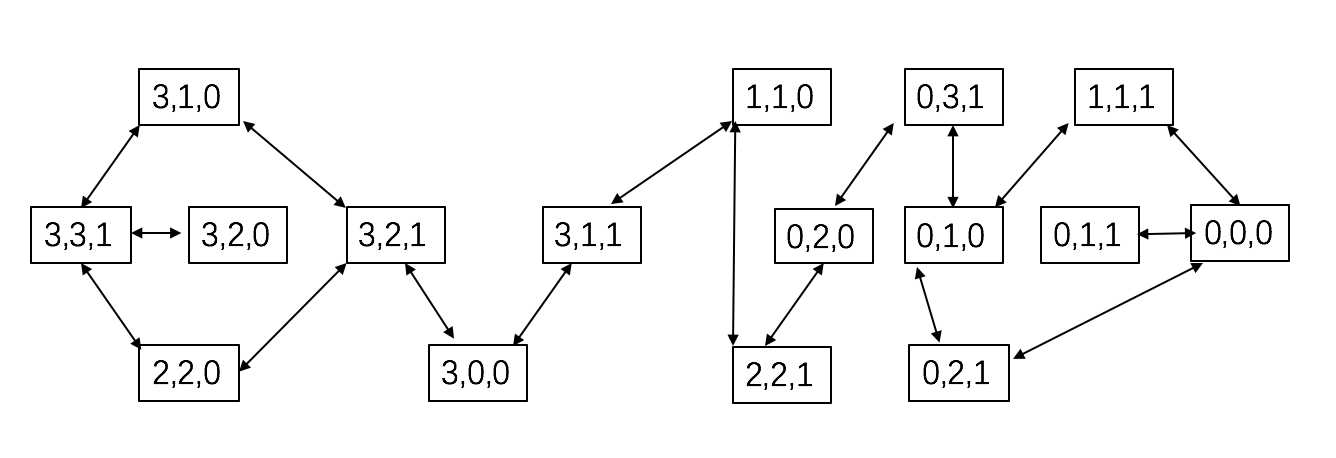
\includegraphics[width=10cm, height = 2.5cm]{1.png}  
\caption*{\small\it The complete state space for this problem}
\end{figure}

\section{Problem 3.21}
\subsection*{a} When all step costs are equal, $g(n) \propto depth(n)$, so uniform-cost search reproduces breadth-first search.
\subsection*{b} 
\begin{itemize}
	\item  \wuhao{Breadth-first is best-first search with $f(n) = depth(n)$ }
	\item  \wuhao{Depth-first search is best -first search with $f(n)=-depth(n)$ }
	\item \wuhao{Uniform-first search is best-first search with $f(n)=g(n)$}

\end{itemize}
\subsection*{c}
Uniform-cost search is $A^*$ search with $h(n)=0$ 


\section{Problem 3.26}
\textbf{a.}  The branching factor is 4. \par
\textbf{b.}The state at depth k form a square rotated at 45 degrees to the grid. So the answer is $4k$  \par
\textbf{c.} WIthout repeated state checking, BFS expands exponentially many nodes, we can computed the exact number :
\begin{quote}
	\centering{$\frac{4^{x+y+1}-4}{3}$}
\end{quote}
\par

\textbf{d.}There are quadratically many states within the square for depth $x+y$, the answer is :
\begin{quote}
	\centering{$2(x+y)(x+y+1)-1$}
\end{quote}
\par

\textbf{e.}The statement is true, because it's manhattan distance metric. \par

\textbf{f.}When $h(n)=0$, since all steps costs are equal, $A^*$ graph search and breadth-first graph search are equal, there are $2(x+y)(x+y+1) - 1$ nodes. \par

\textbf{g.}Removing links may induce detours, which require more steps, so h is an underestimate. So h is still admissible. \par

\textbf{h.}Nonlocal links can reduce the actual path length below the Manhattan distance, so h is may not admissible.


\section{Problem 5.8}
\textbf{a.}  The complete game tree based on the principle can be draw as :
\begin{figure}[ht]
\centering
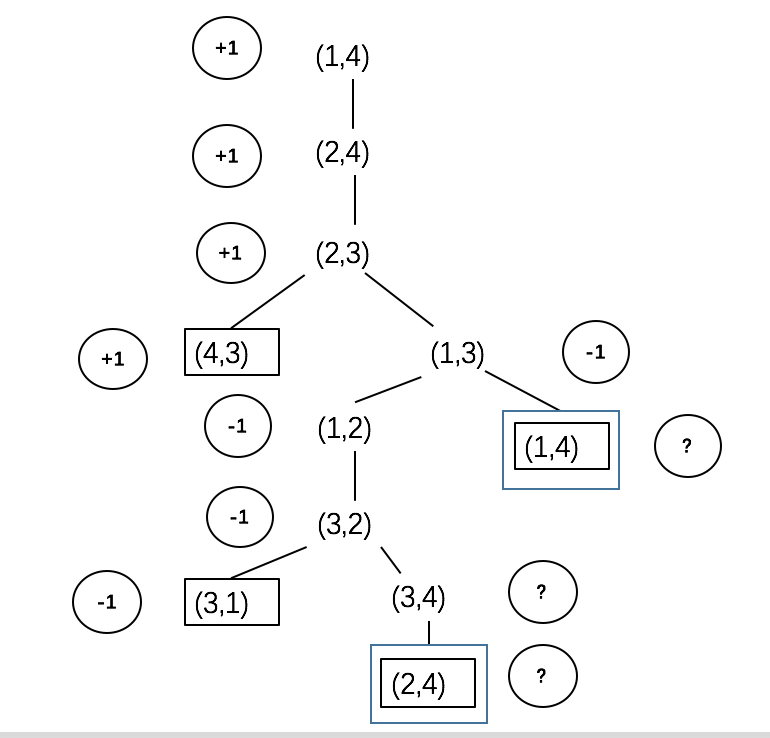
\includegraphics[width=10cm]{2.png}  
\caption*{\small\it The complete game tree}
\end{figure}

\textbf{b.}   The "?" values are handed by assuming that an agent with a choice between winning the game and entering a "?" state. We will always choose to win.
So $\min(-1,?) = -1$
In the same way, we can get that $\max(+1,?) = +1$

\textbf{c.} Standard minimax is depth-first and will go into an infinite loop. It can be fixed by comparing the current state against the stack and if the state is repeated, then return a "?" value, just as drawed in the figure in a.

\textbf{d.} When n = 3, it's a loss for A, and the case for n=4 is a win for A.\par 
For any $n >4$ , the problem can be engaged in a subgame if n-2 on the square 
$[2,\dots,n-1]$. It's clear that if n-2 is win for A, then the game n is also win for A.
By the same line of reasoning, if n-2 is win for B ,then the game n is also win for B. \par 
It's obvious that the player who slated to win the subgame n-2 will never move back to his home square. So we can see that a subgame of $n-2k$ is played on step closer to the loser's home square. All the problem can be turned into the situation for $n=3$ and $n=4$ \par 
So we can prove that A wins if n is even and loses if n is odd.



\section{Problem 5.16}
\textbf{a.} The complete game tree for trivial game can be draw as follow:
\begin{figure}[ht]
	\centering
	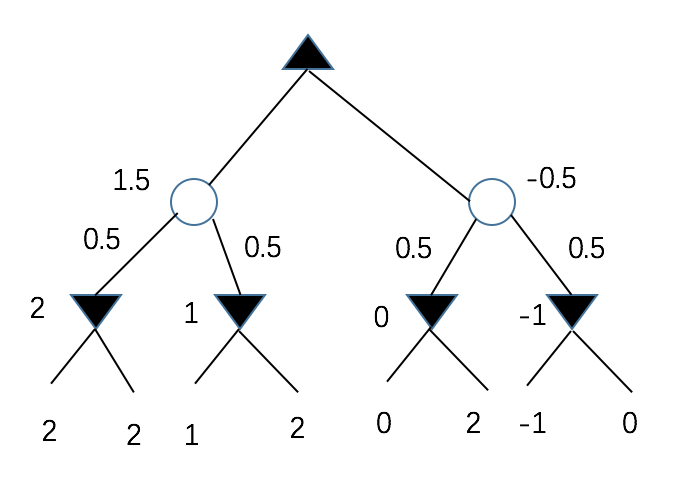
\includegraphics[width=10cm]{3.png}  
	\caption*{\small\it The complete game tree for trivial game}
\end{figure}

\textbf{b.} 
\begin{itemize}
\item  \wuhao {Given nodes 1~6, we would need to look at 7 and 8. If they are both $+\infty$ then the values of the min node and chance node above would be $+\infty$ and the best move will change.} 
\item \wuhao {Given nodes 1~7, we do not need to look at 8, even if it is $+\infty$, the min node can not be worth more than -1. So the chance node above can not be worth more than -0.5, the best move will not change.}
\end{itemize}

\textbf{c.} 
\begin{itemize}
\item \wuhao The worst case is if either of the third and fourth leaves is -2, in which case, chance node above is 0. 
\item \wuhao The best case is where they are both 2, the chance node has value 2. So it must lie between 0 and 2.
\end{itemize}

\textbf{d.}   See the figure in a


%\begin{figure}[ht]
%\centering
%\includegraphics[width=10cm]{pic3.png}  
%\caption*{\small\it Figure 10.4: 4个可能信息以及二值编码的例子}
%\end{figure}


%\begin{itemize}
%\item  \wuhao %{\color{red}{为了传送概率密度函数为$Pr(z)$的随机变量$z$,我们需要$-log_2Pr(z)$位信息}} %\par
%\end{itemize}

%\begin{quote}
%\centering {\color{red}{$length=constant + log\sigma + \frac{(y-\theta)^2}{\sigma^2} + %\frac{\theta^2}{2} \qquad(7.45)$}}
%\end{quote}

\end{document}

